\section{Real-Data}

\subsection{Auto-Correlation}

\def \mywidth {4cm}
\def \myfactor {0.23}

Here follow the ACF and PACF plots for all the real data given by the industrial partner.

\begin{figure}[htp]
	\centering
	\begin{subfigure}{0.23\textwidth}
		\centering
		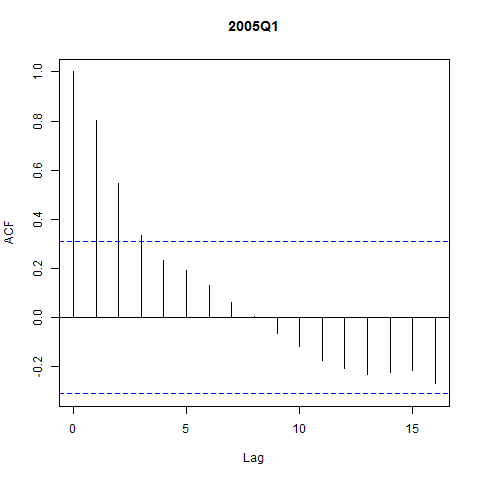
\includegraphics[width= \linewidth]{2005Q1-acf}
		\end{subfigure}
	\begin{subfigure}{0.23\textwidth}
		\centering
		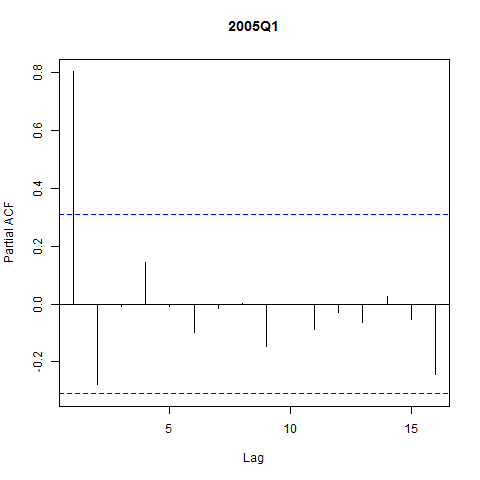
\includegraphics[width=\linewidth]{2005Q1-pacf}
		\end{subfigure}
		\begin{subfigure}{0.23\textwidth}
		\centering
		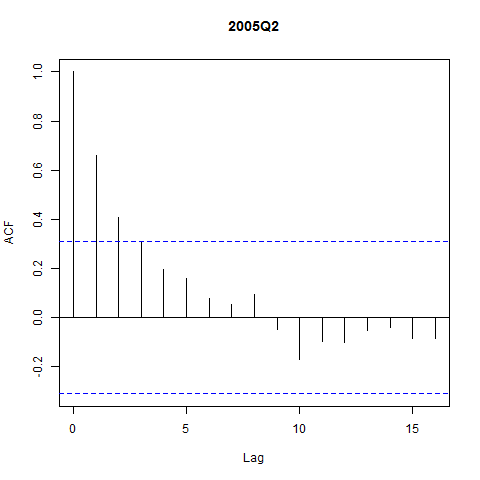
\includegraphics[width= \linewidth]{2005Q2-acf}
	\end{subfigure}
	\begin{subfigure}{0.23\textwidth}
		\centering
		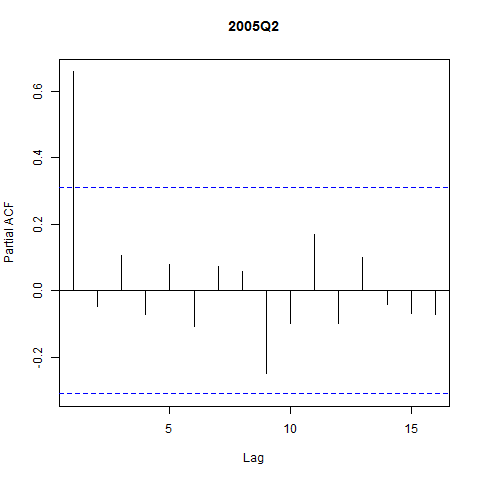
\includegraphics[width=\linewidth]{2005Q2-pacf}
	\end{subfigure}
\end{figure}

\begin{figure}[htp]
	\centering
	\begin{subfigure}{0.23\textwidth}
		\centering
		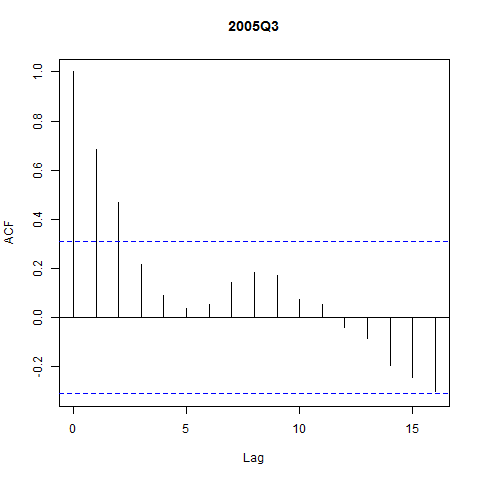
\includegraphics[width= \linewidth]{2005Q3-acf}
	\end{subfigure}
	\begin{subfigure}{0.23\textwidth}
		\centering
		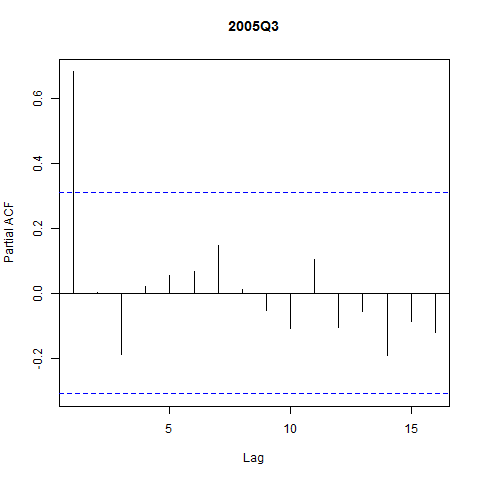
\includegraphics[width=\linewidth]{2005Q3-pacf}
	\end{subfigure}
	\begin{subfigure}{0.23\textwidth}
		\centering
		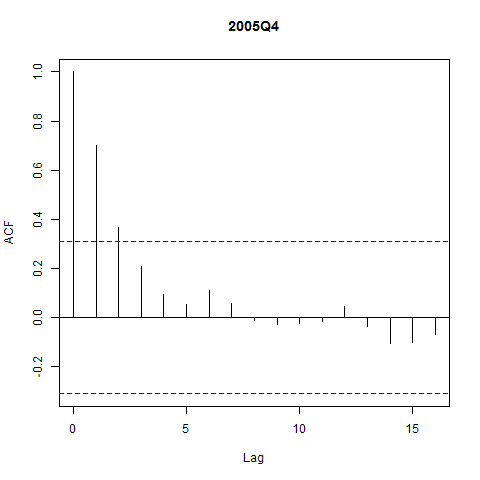
\includegraphics[width= \linewidth]{2005Q4-acf}
	\end{subfigure}
	\begin{subfigure}{0.23\textwidth}
		\centering
		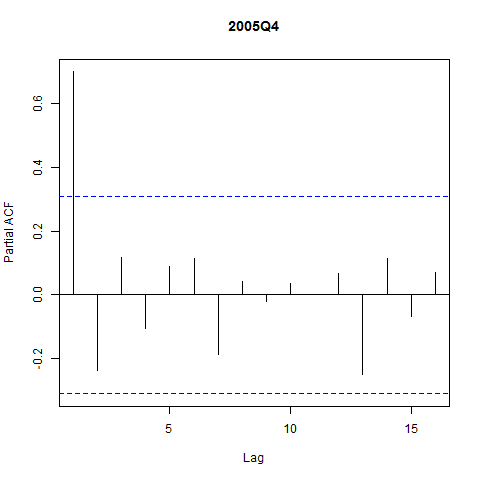
\includegraphics[width=\linewidth]{2005Q4-pacf}
	\end{subfigure}
\end{figure}



\begin{figure}[htp]
	\centering
	\begin{subfigure}{0.23\textwidth}
		\centering
		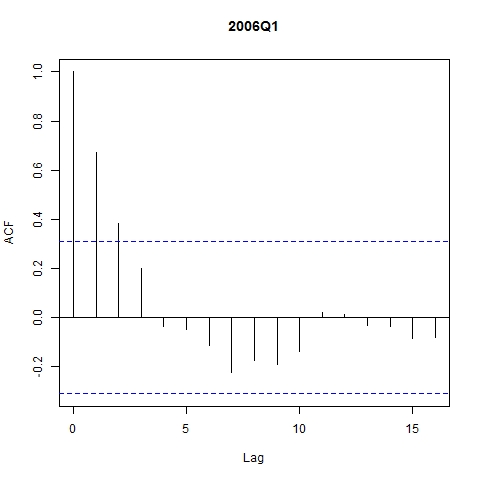
\includegraphics[width= \linewidth]{2006Q1-acf}
	\end{subfigure}
	\begin{subfigure}{0.23\textwidth}
		\centering
		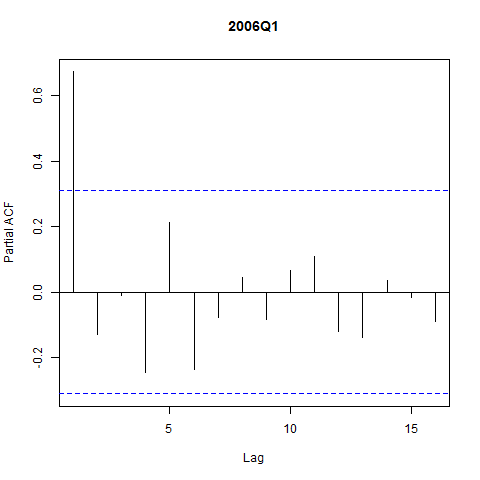
\includegraphics[width=\linewidth]{2006Q1-pacf}
	\end{subfigure}
	\begin{subfigure}{0.23\textwidth}
		\centering
		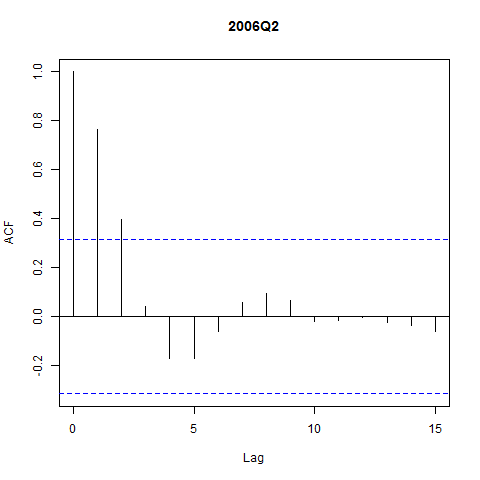
\includegraphics[width= \linewidth]{2006Q2-acf}
	\end{subfigure}
	\begin{subfigure}{0.23\textwidth}
		\centering
		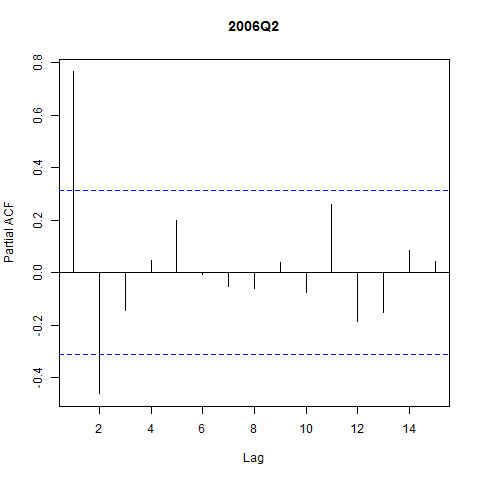
\includegraphics[width=\linewidth]{2006Q2-pacf}
	\end{subfigure}
\end{figure}

\begin{figure}[htp]
	\centering
	\begin{subfigure}{0.23\textwidth}
		\centering
		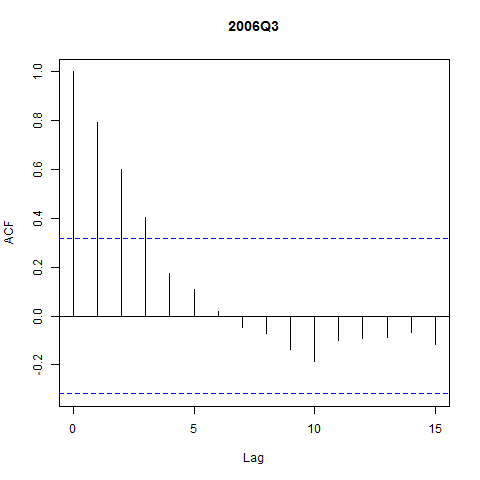
\includegraphics[width= \linewidth]{2006Q3-acf}
	\end{subfigure}
	\begin{subfigure}{0.23\textwidth}
		\centering
		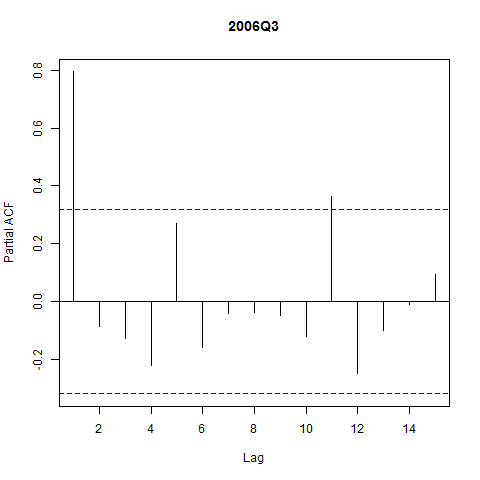
\includegraphics[width=\linewidth]{2006Q3-pacf}
	\end{subfigure}
	\begin{subfigure}{0.23\textwidth}
		\centering
		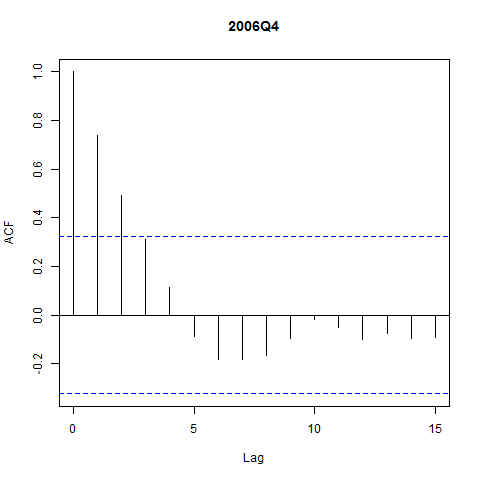
\includegraphics[width= \linewidth]{2006Q4-acf}
	\end{subfigure}
	\begin{subfigure}{0.23\textwidth}
		\centering
		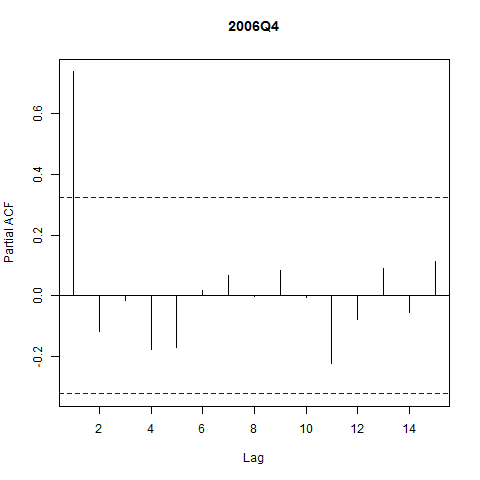
\includegraphics[width=\linewidth]{2006Q4-pacf}
	\end{subfigure}
\end{figure}



\begin{figure}[htp]
	\centering
	\begin{subfigure}{0.23\textwidth}
		\centering
		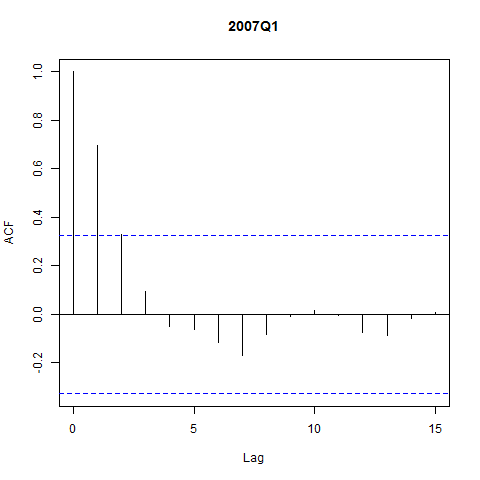
\includegraphics[width= \linewidth]{2007Q1-acf}
	\end{subfigure}
	\begin{subfigure}{0.23\textwidth}
		\centering
		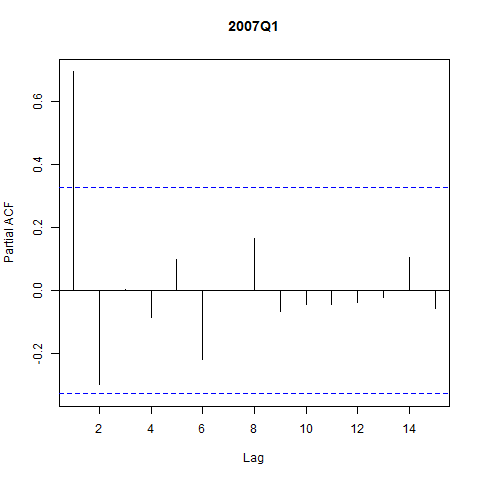
\includegraphics[width=\linewidth]{2007Q1-pacf}
	\end{subfigure}
	\begin{subfigure}{0.23\textwidth}
		\centering
		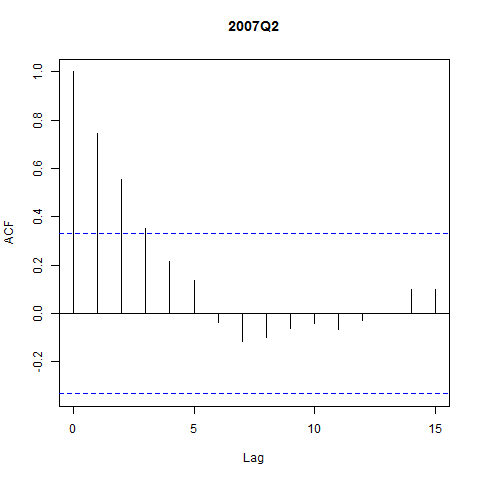
\includegraphics[width= \linewidth]{2007Q2-acf}
	\end{subfigure}
	\begin{subfigure}{0.23\textwidth}
		\centering
		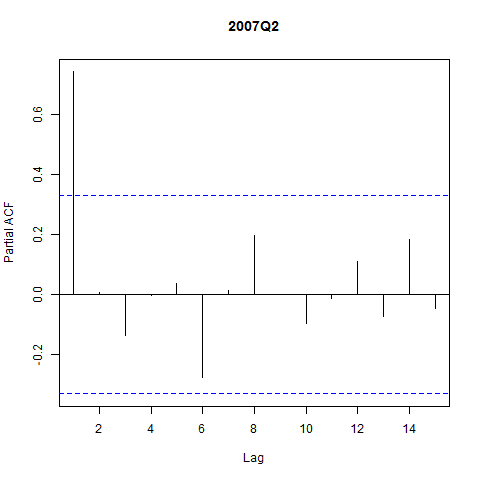
\includegraphics[width=\linewidth]{2007Q2-pacf}
	\end{subfigure}
\end{figure}

\begin{figure}[htp]
	\centering
	\begin{subfigure}{0.23\textwidth}
		\centering
		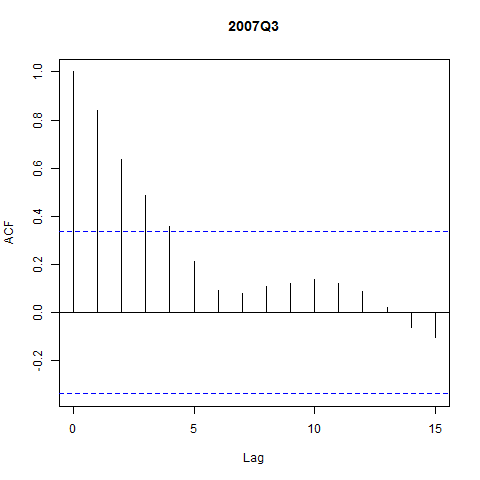
\includegraphics[width= \linewidth]{2007Q3-acf}
	\end{subfigure}
	\begin{subfigure}{0.23\textwidth}
		\centering
		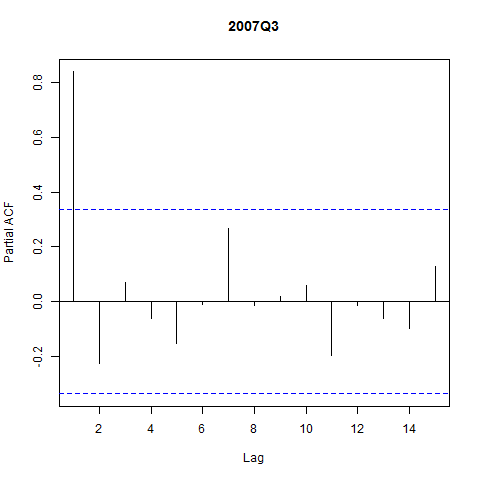
\includegraphics[width=\linewidth]{2007Q3-pacf}
	\end{subfigure}
	\begin{subfigure}{0.23\textwidth}
		\centering
		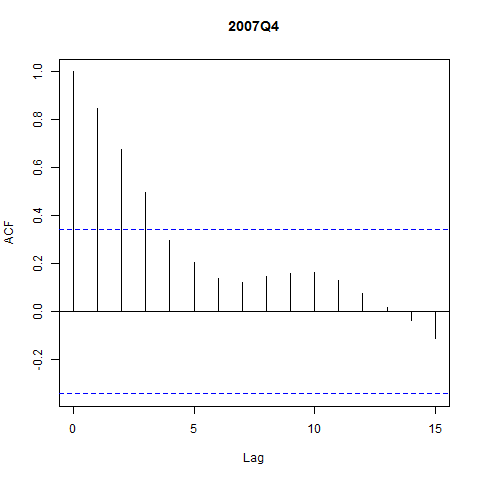
\includegraphics[width= \linewidth]{2007Q4-acf}
	\end{subfigure}
	\begin{subfigure}{0.23\textwidth}
		\centering
		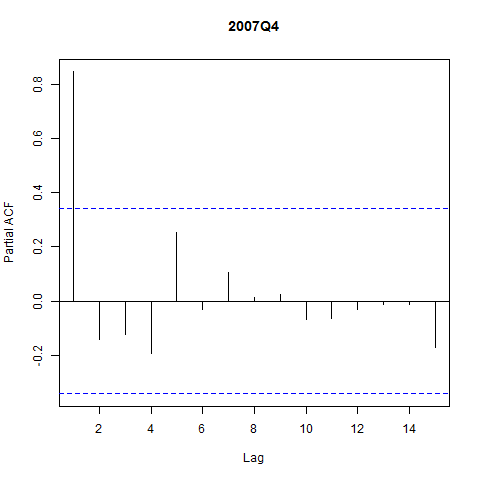
\includegraphics[width=\linewidth]{2007Q4-pacf}
	\end{subfigure}
\end{figure}



\begin{figure}[htp]
	\centering
	\begin{subfigure}{0.23\textwidth}
		\centering
		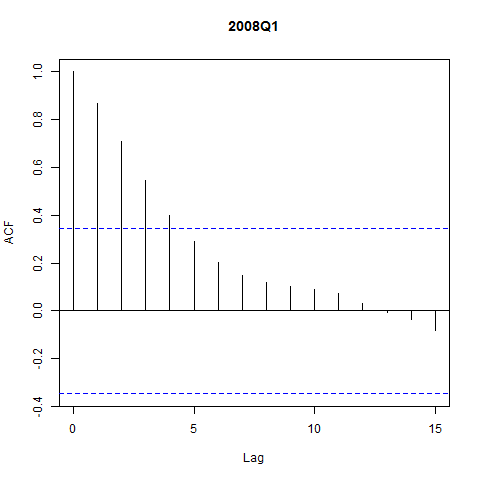
\includegraphics[width= \linewidth]{2008Q1-acf}
	\end{subfigure}
	\begin{subfigure}{0.23\textwidth}
		\centering
		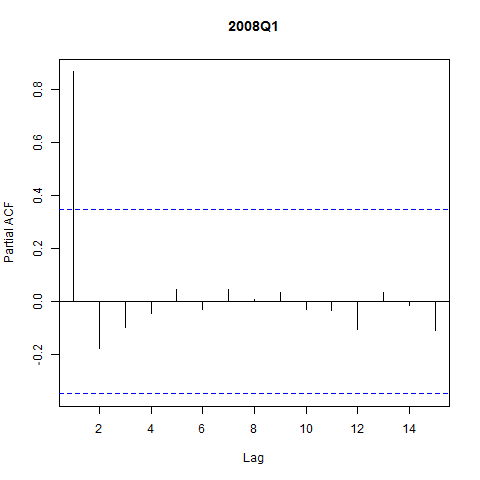
\includegraphics[width=\linewidth]{2008Q1-pacf}
	\end{subfigure}
	\begin{subfigure}{0.23\textwidth}
		\centering
		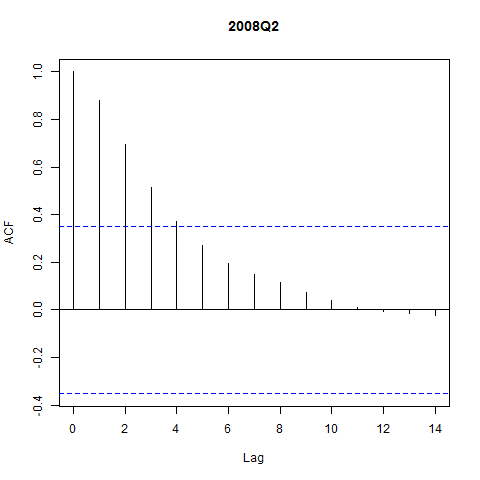
\includegraphics[width= \linewidth]{2008Q2-acf}
	\end{subfigure}
	\begin{subfigure}{0.23\textwidth}
		\centering
		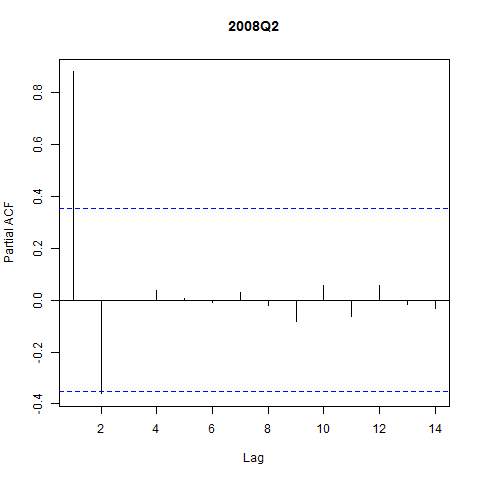
\includegraphics[width=\linewidth]{2008Q2-pacf}
	\end{subfigure}
\end{figure}

\begin{figure}[htp]
	\centering
	\begin{subfigure}{0.23\textwidth}
		\centering
		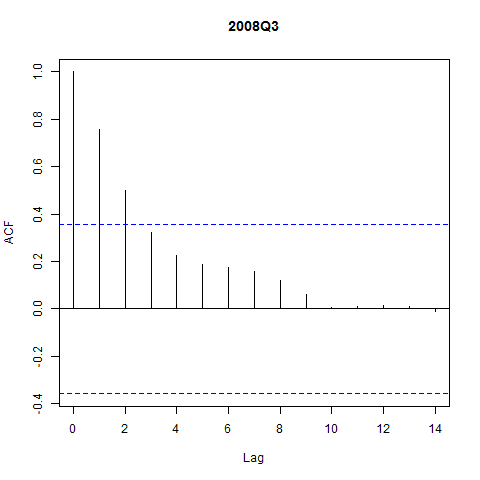
\includegraphics[width= \linewidth]{2008Q3-acf}
	\end{subfigure}
	\begin{subfigure}{0.23\textwidth}
		\centering
		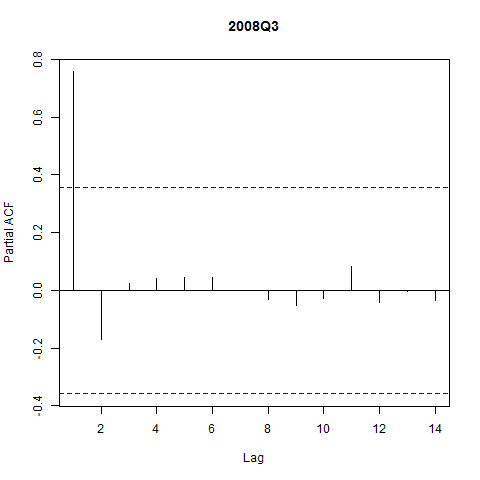
\includegraphics[width=\linewidth]{2008Q3-pacf}
	\end{subfigure}
	\begin{subfigure}{0.23\textwidth}
		\centering
		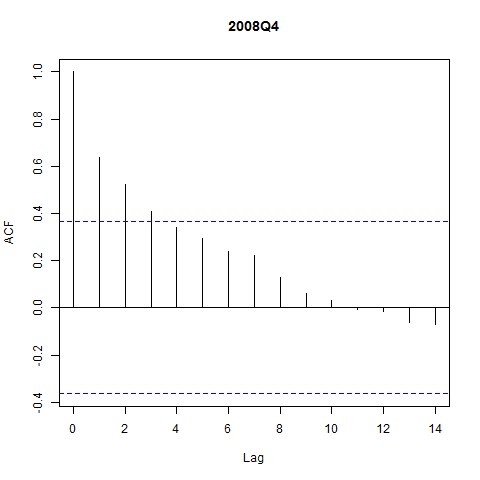
\includegraphics[width= \linewidth]{2008Q4-acf}
	\end{subfigure}
	\begin{subfigure}{0.23\textwidth}
		\centering
		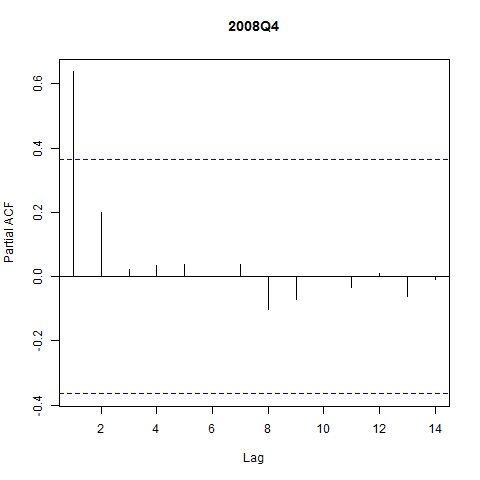
\includegraphics[width=\linewidth]{2008Q4-pacf}
	\end{subfigure}
\end{figure}



\begin{figure}[htp]
	\centering
	\begin{subfigure}{0.23\textwidth}
		\centering
		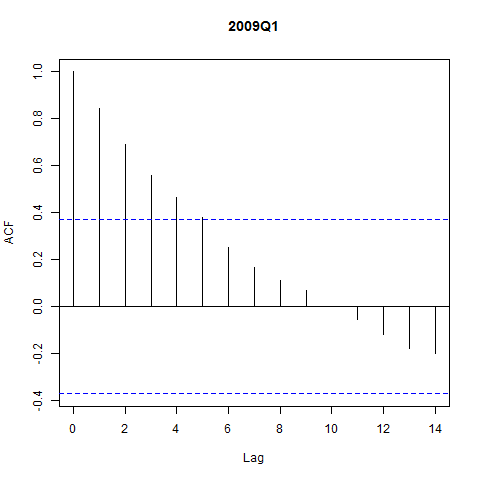
\includegraphics[width= \linewidth]{2009Q1-acf}
	\end{subfigure}
	\begin{subfigure}{0.23\textwidth}
		\centering
		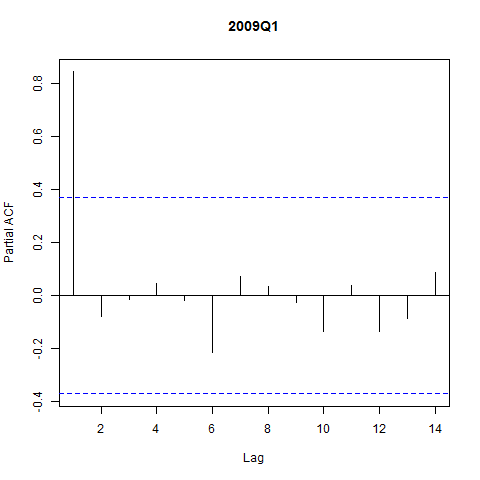
\includegraphics[width=\linewidth]{2009Q1-pacf}
	\end{subfigure}
	\begin{subfigure}{0.23\textwidth}
		\centering
		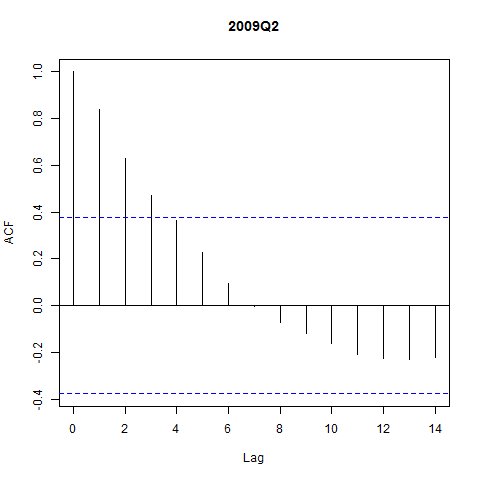
\includegraphics[width= \linewidth]{2009Q2-acf}
	\end{subfigure}
	\begin{subfigure}{0.23\textwidth}
		\centering
		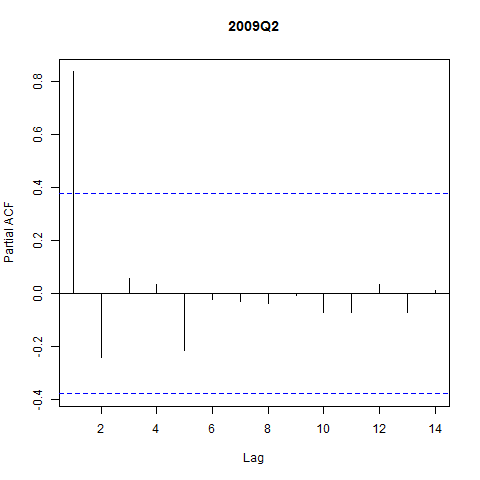
\includegraphics[width=\linewidth]{2009Q2-pacf}
	\end{subfigure}
\end{figure}

\begin{figure}[htp]
	\centering
	\begin{subfigure}{0.23\textwidth}
		\centering
		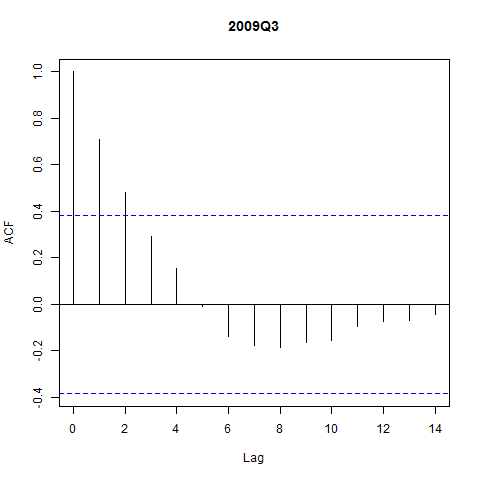
\includegraphics[width= \linewidth]{2009Q3-acf}
	\end{subfigure}
	\begin{subfigure}{0.23\textwidth}
		\centering
		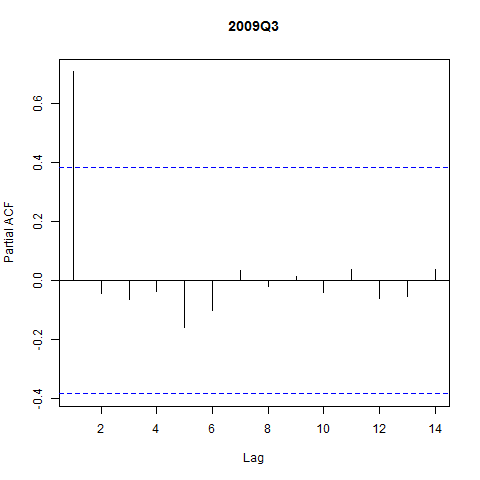
\includegraphics[width=\linewidth]{2009Q3-pacf}
	\end{subfigure}
	\begin{subfigure}{0.23\textwidth}
		\centering
		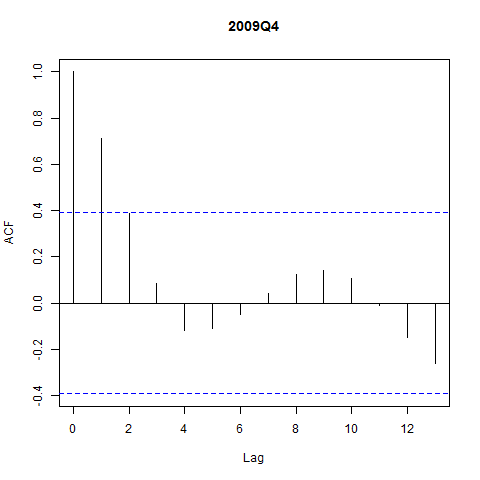
\includegraphics[width= \linewidth]{2009Q4-acf}
	\end{subfigure}
	\begin{subfigure}{0.23\textwidth}
		\centering
		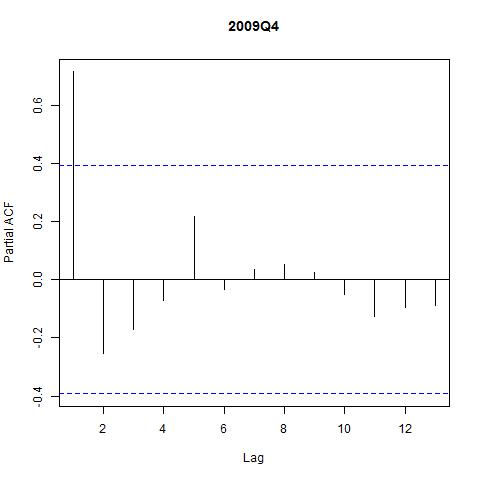
\includegraphics[width=\linewidth]{2009Q4-pacf}
	\end{subfigure}
\end{figure}



\begin{figure}[htp]
	\centering
	\begin{subfigure}{0.23\textwidth}
		\centering
		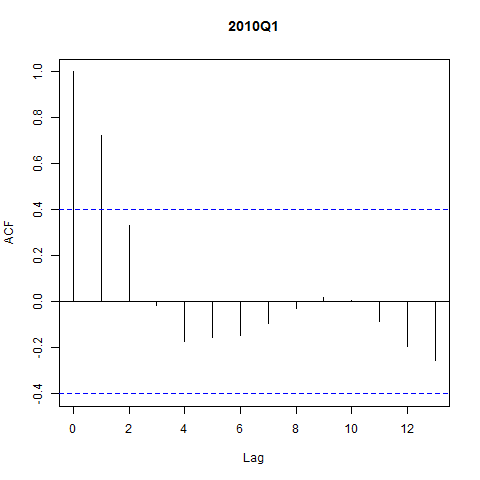
\includegraphics[width= \linewidth]{2010Q1-acf}
	\end{subfigure}
	\begin{subfigure}{0.23\textwidth}
		\centering
		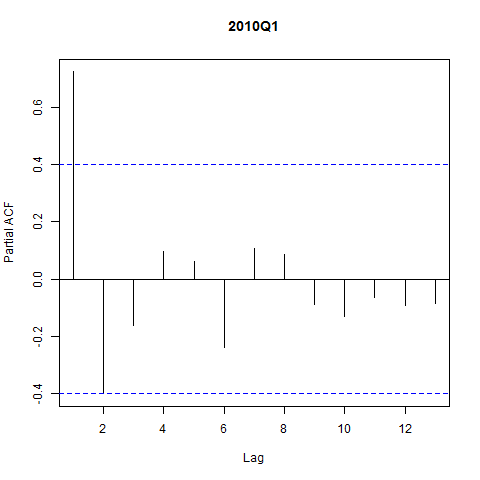
\includegraphics[width=\linewidth]{2010Q1-pacf}
	\end{subfigure}
	\begin{subfigure}{0.23\textwidth}
		\centering
		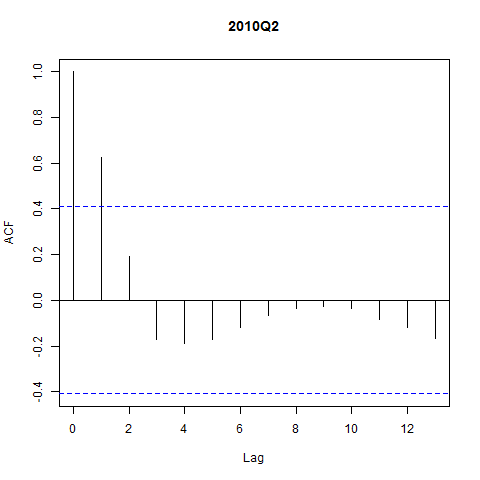
\includegraphics[width= \linewidth]{2010Q2-acf}
	\end{subfigure}
	\begin{subfigure}{0.23\textwidth}
		\centering
		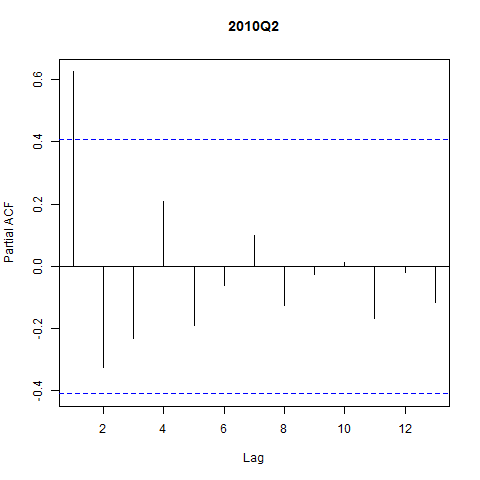
\includegraphics[width=\linewidth]{2010Q2-pacf}
	\end{subfigure}
\end{figure}

\begin{figure}[htp]
	\centering
	\begin{subfigure}{0.23\textwidth}
		\centering
		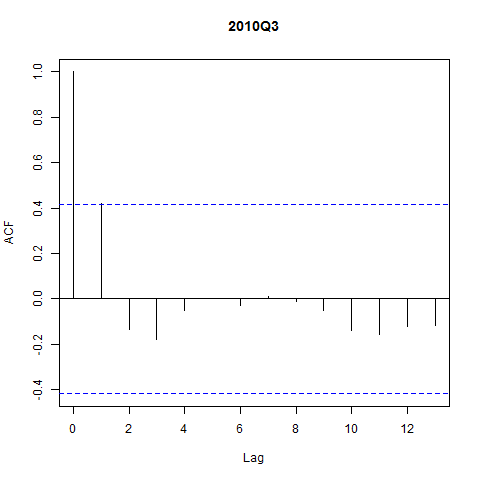
\includegraphics[width= \linewidth]{2010Q3-acf}
	\end{subfigure}
	\begin{subfigure}{0.23\textwidth}
		\centering
		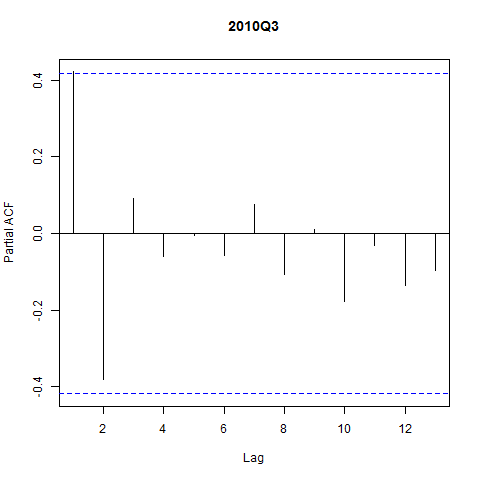
\includegraphics[width=\linewidth]{2010Q3-pacf}
	\end{subfigure}
	\begin{subfigure}{0.23\textwidth}
		\centering
		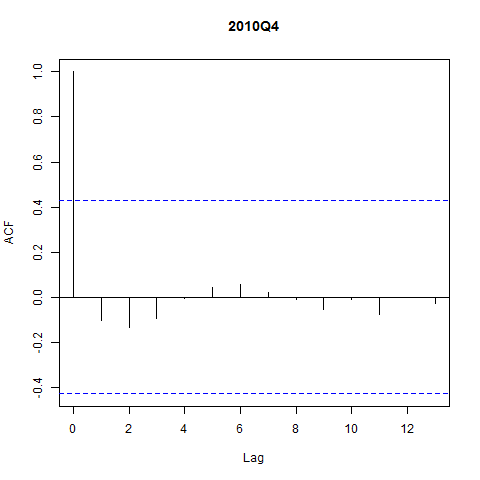
\includegraphics[width= \linewidth]{2010Q4-acf}
	\end{subfigure}
	\begin{subfigure}{0.23\textwidth}
		\centering
		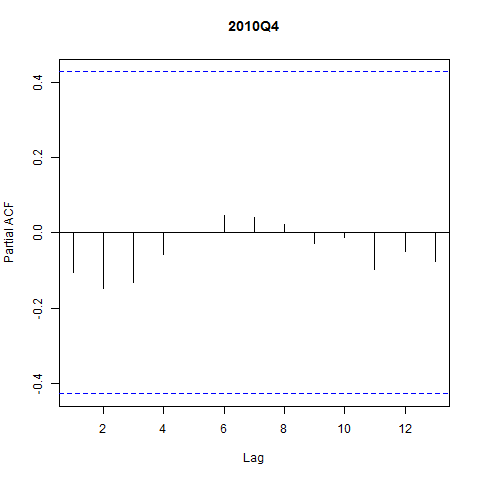
\includegraphics[width=\linewidth]{2010Q4-pacf}
	\end{subfigure}
\end{figure}



\begin{figure}[htp]
	\centering
	\begin{subfigure}{0.23\textwidth}
		\centering
		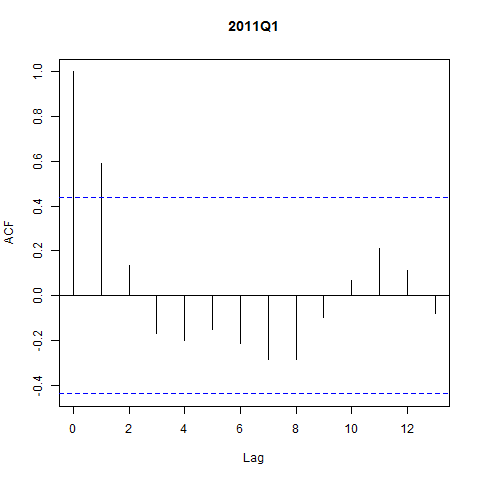
\includegraphics[width= \linewidth]{2011Q1-acf}
	\end{subfigure}
	\begin{subfigure}{0.23\textwidth}
		\centering
		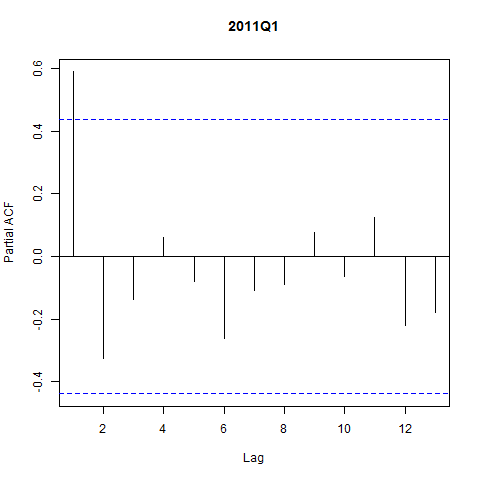
\includegraphics[width=\linewidth]{2011Q1-pacf}
	\end{subfigure}
	\begin{subfigure}{0.23\textwidth}
		\centering
		\includegraphics[width= \linewidth]{2011Q2-acf}
	\end{subfigure}
	\begin{subfigure}{0.23\textwidth}
		\centering
		\includegraphics[width=\linewidth]{2011Q2-pacf}
	\end{subfigure}
\end{figure}

\begin{figure}[htp]
	\centering
	\begin{subfigure}{0.23\textwidth}
		\centering
		\includegraphics[width= \linewidth]{2011Q3-acf}
	\end{subfigure}
	\begin{subfigure}{0.23\textwidth}
		\centering
		\includegraphics[width=\linewidth]{2011Q3-pacf}
	\end{subfigure}
	\begin{subfigure}{0.23\textwidth}
		\centering
		\includegraphics[width= \linewidth]{2011Q4-acf}
	\end{subfigure}
	\begin{subfigure}{0.23\textwidth}
		\centering
		\includegraphics[width=\linewidth]{2011Q4-pacf}
	\end{subfigure}
\end{figure}



\begin{figure}[htp]
	\centering
	\begin{subfigure}{0.23\textwidth}
		\centering
		\includegraphics[width= \linewidth]{2012Q1-acf}
	\end{subfigure}
	\begin{subfigure}{0.23\textwidth}
		\centering
		\includegraphics[width=\linewidth]{2012Q1-pacf}
	\end{subfigure}
	\begin{subfigure}{0.23\textwidth}
		\centering
		\includegraphics[width= \linewidth]{2012Q2-acf}
	\end{subfigure}
	\begin{subfigure}{0.23\textwidth}
		\centering
		\includegraphics[width=\linewidth]{2012Q2-pacf}
	\end{subfigure}
\end{figure}

\begin{figure}[htp]
	\centering
	\begin{subfigure}{0.23\textwidth}
		\centering
		\includegraphics[width= \linewidth]{2012Q3-acf}
	\end{subfigure}
	\begin{subfigure}{0.23\textwidth}
		\centering
		\includegraphics[width=\linewidth]{2012Q3-pacf}
	\end{subfigure}
	\begin{subfigure}{0.23\textwidth}
		\centering
		\includegraphics[width= \linewidth]{2012Q4-acf}
	\end{subfigure}
	\begin{subfigure}{0.23\textwidth}
		\centering
		\includegraphics[width=\linewidth]{2012Q4-pacf}
	\end{subfigure}
\end{figure}



\begin{figure}[htp]
	\centering
	\begin{subfigure}{0.23\textwidth}
		\centering
		\includegraphics[width= \linewidth]{2013Q1-acf}
	\end{subfigure}
	\begin{subfigure}{0.23\textwidth}
		\centering
		\includegraphics[width=\linewidth]{2013Q1-pacf}
	\end{subfigure}
	\begin{subfigure}{0.23\textwidth}
		\centering
		\includegraphics[width= \linewidth]{2013Q2-acf}
	\end{subfigure}
	\begin{subfigure}{0.23\textwidth}
		\centering
		\includegraphics[width=\linewidth]{2013Q2-pacf}
	\end{subfigure}
\end{figure}

\begin{figure}[htp]
	\centering
	\begin{subfigure}{0.23\textwidth}
		\centering
		\includegraphics[width= \linewidth]{2013Q3-acf}
	\end{subfigure}
	\begin{subfigure}{0.23\textwidth}
		\centering
		\includegraphics[width=\linewidth]{2013Q3-pacf}
	\end{subfigure}
	\begin{subfigure}{0.23\textwidth}
		\centering
		\includegraphics[width= \linewidth]{2013Q4-acf}
	\end{subfigure}
	\begin{subfigure}{0.23\textwidth}
		\centering
		\includegraphics[width=\linewidth]{2013Q4-pacf}
	\end{subfigure}
\end{figure}



\begin{figure}[htp]
	\centering
	\begin{subfigure}{0.23\textwidth}
		\centering
		\includegraphics[width= \linewidth]{2014Q1-acf}
	\end{subfigure}
	\begin{subfigure}{0.23\textwidth}
		\centering
		\includegraphics[width=\linewidth]{2014Q1-pacf}
	\end{subfigure}
	\begin{subfigure}{0.23\textwidth}
		\centering
		\includegraphics[width= \linewidth]{2014Q2-acf}
	\end{subfigure}
	\begin{subfigure}{0.23\textwidth}
		\centering
		\includegraphics[width=\linewidth]{2014Q2-pacf}
	\end{subfigure}
\end{figure}

\begin{figure}[htp]
	\centering
	\begin{subfigure}{0.23\textwidth}
		\centering
		\includegraphics[width= \linewidth]{2014Q3-acf}
	\end{subfigure}
	\begin{subfigure}{0.23\textwidth}
		\centering
		\includegraphics[width=\linewidth]{2014Q3-pacf}
	\end{subfigure}
	\begin{subfigure}{0.23\textwidth}
		\centering
		\includegraphics[width= \linewidth]{2014Q4-acf}
	\end{subfigure}
	\begin{subfigure}{0.23\textwidth}
		\centering
		\includegraphics[width=\linewidth]{2014Q4-pacf}
	\end{subfigure}
\end{figure}


\begin{figure}[htp]
	\centering
	\begin{subfigure}{0.23\textwidth}
		\centering
		\includegraphics[width= \linewidth]{2015Q1-acf}
	\end{subfigure}
	\begin{subfigure}{0.23\textwidth}
		\centering
		\includegraphics[width=\linewidth]{2015Q1-pacf}
	\end{subfigure}
	\begin{subfigure}{0.23\textwidth}
		\centering
		\includegraphics[width= \linewidth]{2015Q2-acf}
	\end{subfigure}
	\begin{subfigure}{0.23\textwidth}
		\centering
		\includegraphics[width=\linewidth]{2015Q2-pacf}
	\end{subfigure}
\end{figure}

\begin{figure}[htp]
	\centering
	\begin{subfigure}{0.23\textwidth}
		\centering
		\includegraphics[width= \linewidth]{2015Q3-acf}
	\end{subfigure}
	\begin{subfigure}{0.23\textwidth}
		\centering
		\includegraphics[width=\linewidth]{2015Q3-pacf}
	\end{subfigure}
\end{figure}

\pagebreak


\subsection{Time-Series Plots}

\begin{figure}[htp]
	\centering
	\begin{subfigure}{0.75\textwidth}
		\centering
		\includegraphics[width= \linewidth]{panel_graph}
	\end{subfigure}
	\caption{Time series plot of all real data.}
\end{figure}

\section{Simulated Data}

As was discussed in greater detail in Chapter 4, the following is ACF, PACF and time series plots of the processes generated for the Monte Carlo simulations.

\subsection{Auto-Correlation}

The following is a collection of Auto-Correlation and Partial Auto-Correlation function graphs for the processes simulated using the Monte Carlo method for cases where $\rho = 0.5$, $\rho = 0.75$, $\rho = 0.99$, and $\rho = 1$.

\subsubsection{$CASE: \rho = 0.5$}

\begin{figure}[htp]
	\centering
	\begin{subfigure}{0.23\textwidth}
		\centering
		\includegraphics[width= \linewidth]{10-05-acf}
	\end{subfigure}
	\begin{subfigure}{0.23\textwidth}
		\centering
		\includegraphics[width=\linewidth]{10-05-pacf}
	\end{subfigure}
	\begin{subfigure}{0.23\textwidth}
		\centering
		\includegraphics[width= \linewidth]{20-05-acf}
	\end{subfigure}
	\begin{subfigure}{0.23\textwidth}
		\centering
		\includegraphics[width=\linewidth]{20-05-pacf}
	\end{subfigure}
\end{figure}

\begin{figure}[htp]
	\centering
	\begin{subfigure}{0.23\textwidth}
		\centering
		\includegraphics[width= \linewidth]{100-05-acf}
	\end{subfigure}
	\begin{subfigure}{0.23\textwidth}
		\centering
		\includegraphics[width=\linewidth]{100-05-pacf}
	\end{subfigure}
	\begin{subfigure}{0.23\textwidth}
		\centering
		\includegraphics[width= \linewidth]{500-05-acf}
	\end{subfigure}
	\begin{subfigure}{0.23\textwidth}
		\centering
		\includegraphics[width=\linewidth]{500-05-pacf}
	\end{subfigure}
\end{figure}

\pagebreak

\subsubsection{$CASE: \rho = 0.75$}

\begin{figure}[htp]
	\centering
	\begin{subfigure}{0.23\textwidth}
		\centering
		\includegraphics[width= \linewidth]{10-075-acf}
	\end{subfigure}
	\begin{subfigure}{0.23\textwidth}
		\centering
		\includegraphics[width=\linewidth]{10-075-pacf}
	\end{subfigure}
	\begin{subfigure}{0.23\textwidth}
		\centering
		\includegraphics[width= \linewidth]{20-075-acf}
	\end{subfigure}
	\begin{subfigure}{0.23\textwidth}
		\centering
		\includegraphics[width=\linewidth]{20-075-pacf}
	\end{subfigure}
\end{figure}

\begin{figure}[htp]
	\centering
	\begin{subfigure}{0.23\textwidth}
		\centering
		\includegraphics[width= \linewidth]{100-075-acf}
	\end{subfigure}
	\begin{subfigure}{0.23\textwidth}
		\centering
		\includegraphics[width=\linewidth]{100-075-pacf}
	\end{subfigure}
	\begin{subfigure}{0.23\textwidth}
		\centering
		\includegraphics[width= \linewidth]{500-075-acf}
	\end{subfigure}
	\begin{subfigure}{0.23\textwidth}
		\centering
		\includegraphics[width=\linewidth]{500-075-pacf}
	\end{subfigure}
\end{figure}

\subsubsection{$CASE: \rho = 0.9$}

\begin{figure}[htp]
	\centering
	\begin{subfigure}{0.23\textwidth}
		\centering
		\includegraphics[width= \linewidth]{10-09-acf}
	\end{subfigure}
	\begin{subfigure}{0.23\textwidth}
		\centering
		\includegraphics[width=\linewidth]{10-09-pacf}
	\end{subfigure}
	\begin{subfigure}{0.23\textwidth}
		\centering
		\includegraphics[width= \linewidth]{20-09-acf}
	\end{subfigure}
	\begin{subfigure}{0.23\textwidth}
		\centering
		\includegraphics[width=\linewidth]{20-09-pacf}
	\end{subfigure}
\end{figure}

\begin{figure}[htp]
	\centering
	\begin{subfigure}{0.23\textwidth}
		\centering
		\includegraphics[width= \linewidth]{100-09-acf}
	\end{subfigure}
	\begin{subfigure}{0.23\textwidth}
		\centering
		\includegraphics[width=\linewidth]{100-09-pacf}
	\end{subfigure}
	\begin{subfigure}{0.23\textwidth}
		\centering
		\includegraphics[width= \linewidth]{500-09-acf}
	\end{subfigure}
	\begin{subfigure}{0.23\textwidth}
		\centering
		\includegraphics[width=\linewidth]{500-09-pacf}
	\end{subfigure}
\end{figure}

\pagebreak

\subsubsection{$CASE: \rho = 1$}

\begin{figure}[htp]
	\centering
	\begin{subfigure}{0.23\textwidth}
		\centering
		\includegraphics[width= \linewidth]{10-100-acf}
	\end{subfigure}
	\begin{subfigure}{0.23\textwidth}
		\centering
		\includegraphics[width=\linewidth]{10-100-pacf}
	\end{subfigure}
	\begin{subfigure}{0.23\textwidth}
		\centering
		\includegraphics[width= \linewidth]{20-1-acf}
	\end{subfigure}
	\begin{subfigure}{0.23\textwidth}
		\centering
		\includegraphics[width=\linewidth]{20-1-pacf}
	\end{subfigure}
\end{figure}

\begin{figure}[htp]
	\centering
	\begin{subfigure}{0.23\textwidth}
		\centering
		\includegraphics[width= \linewidth]{100-1-acf}
	\end{subfigure}
	\begin{subfigure}{0.23\textwidth}
		\centering
		\includegraphics[width=\linewidth]{100-1-pacf}
	\end{subfigure}
	\begin{subfigure}{0.23\textwidth}
		\centering
		\includegraphics[width= \linewidth]{500-1-acf}
	\end{subfigure}
	\begin{subfigure}{0.23\textwidth}
		\centering
		\includegraphics[width=\linewidth]{500-1-pacf}
	\end{subfigure}
\end{figure}


\subsection{Time-Series Plots}

The following are the time series plots for $ T = 10$, $ T = 20$, $ T = 100$ and $ T = 500$ for $\rho = 0.5$, $\rho = 0.75$, $\rho = 0.9$ and $\rho = 1$.

\subsubsection{$CASE: \rho = 0.5$}

\begin{figure}[htp]
	\centering
	\begin{subfigure}{0.23\textwidth}
		\centering
		\includegraphics[width= \linewidth]{10-05-plot}
	\end{subfigure}
	\begin{subfigure}{0.23\textwidth}
		\centering
		\includegraphics[width=\linewidth]{20-05-plot}
	\end{subfigure}
	\begin{subfigure}{0.23\textwidth}
		\centering
		\includegraphics[width= \linewidth]{100-05-plot}
	\end{subfigure}
	\begin{subfigure}{0.23\textwidth}
		\centering
		\includegraphics[width=\linewidth]{500-05-plot}
	\end{subfigure}
\end{figure}

\subsubsection{$CASE: \rho = 0.75$}

\begin{figure}[htp]
	\centering
	\begin{subfigure}{0.23\textwidth}
		\centering
		\includegraphics[width= \linewidth]{10-075-plot}
	\end{subfigure}
	\begin{subfigure}{0.23\textwidth}
		\centering
		\includegraphics[width=\linewidth]{20-075-plot}
	\end{subfigure}
	\begin{subfigure}{0.23\textwidth}
		\centering
		\includegraphics[width= \linewidth]{100-075-plot}
	\end{subfigure}
	\begin{subfigure}{0.23\textwidth}
		\centering
		\includegraphics[width=\linewidth]{500-075-plot}
	\end{subfigure}
\end{figure}

\pagebreak

\subsubsection{$CASE: \rho = 0.9$}

\begin{figure}[htp]
	
	\begin{subfigure}{0.23\textwidth}
		\centering
		\includegraphics[width= \linewidth]{10-09-plot}
	\end{subfigure}
	\begin{subfigure}{0.23\textwidth}
		\centering
		\includegraphics[width=\linewidth]{20-09-plot}
	\end{subfigure}
	\begin{subfigure}{0.23\textwidth}
		\centering
		\includegraphics[width= \linewidth]{100-09-plot}
	\end{subfigure}
	\begin{subfigure}{0.23\textwidth}
		\centering
		\includegraphics[width=\linewidth]{500-09-plot}
	\end{subfigure}
\end{figure}

\subsubsection{$CASE: \rho = 1$}

\begin{figure}[htp]
	\centering
	\begin{subfigure}{0.23\textwidth}
		\centering
		\includegraphics[width= \linewidth]{10-100-plot}
	\end{subfigure}
	\begin{subfigure}{0.23\textwidth}
		\centering
		\includegraphics[width=\linewidth]{20-1-plot}
	\end{subfigure}
	\begin{subfigure}{0.23\textwidth}
		\centering
		\includegraphics[width= \linewidth]{100-1-plot}
	\end{subfigure}
	\begin{subfigure}{0.23\textwidth}
		\centering
		\includegraphics[width=\linewidth]{500-1-plot}
	\end{subfigure}
\end{figure} 

\section{Results in Full}

\subsection{Full Panel Test Output}
\lstset{basicstyle=\tiny\tt,style=myStyle,breaklines=true,}

\begin{lstlisting}[language=R]


=========================================================================
Created panel of 2 individuals and 39 observations.
-------------------------------------------------------------------------

Levin-Lin-Chu Result:   Non-Stationary  @  0.357935269016302

Maddala-Wu Result:      Non-Stationary  @  0.821140745455104

IPS Result:     Non-Stationary  @  0.665238951063704

ADF      Stationary: 0  Non-Stationary: 2

PP       Stationary: 0  Non-Stationary: 2

=========================================================================
Created panel of 3 individuals and 39 observations.
-------------------------------------------------------------------------

Levin-Lin-Chu Result:   Non-Stationary  @  0.221880094700225

Maddala-Wu Result:      Non-Stationary  @  0.935052474835083

IPS Result:     Non-Stationary  @  0.683545452570764

ADF      Stationary: 0  Non-Stationary: 3

PP       Stationary: 0  Non-Stationary: 3

=========================================================================
Created panel of 4 individuals and 39 observations.
-------------------------------------------------------------------------

Levin-Lin-Chu Result:   Non-Stationary  @  0.280340127531492

Maddala-Wu Result:      Non-Stationary  @  0.94797897059072

IPS Result:     Non-Stationary  @  0.639211255315669

ADF      Stationary: 0  Non-Stationary: 4

PP       Stationary: 0  Non-Stationary: 4

=========================================================================
Created panel of 5 individuals and 39 observations.
-------------------------------------------------------------------------

Levin-Lin-Chu Result:   Non-Stationary  @  0.529629326002611

Maddala-Wu Result:      Non-Stationary  @  0.9848425562163

IPS Result:     Non-Stationary  @  0.340347819163327

ADF      Stationary: 0  Non-Stationary: 5

PP       Stationary: 0  Non-Stationary: 5

=========================================================================
Created panel of 6 individuals and 38 observations.
-------------------------------------------------------------------------

Levin-Lin-Chu Result:   Stationary  @  0.0653993707410805

Maddala-Wu Result:      Non-Stationary  @  0.799997287818515

IPS Result:     Non-Stationary  @  0.864948676868659

ADF      Stationary: 0  Non-Stationary: 6

PP       Stationary: 0  Non-Stationary: 6

=========================================================================
Created panel of 7 individuals and 37 observations.
-------------------------------------------------------------------------

Levin-Lin-Chu Result:   Stationary  @  0.026441106340915

Maddala-Wu Result:      Non-Stationary  @  0.759238552254934

IPS Result:     Non-Stationary  @  0.897189453363048

ADF      Stationary: 0  Non-Stationary: 7

PP       Stationary: 0  Non-Stationary: 7

=========================================================================
Created panel of 8 individuals and 36 observations.
-------------------------------------------------------------------------

Levin-Lin-Chu Result:   Stationary  @  0.00355709761805292

Maddala-Wu Result:      Non-Stationary  @  0.632340076581622

IPS Result:     Non-Stationary  @  0.64897544996669

ADF      Stationary: 8  Non-Stationary: 0

PP       Stationary: 0  Non-Stationary: 8

=========================================================================
Created panel of 9 individuals and 35 observations.
-------------------------------------------------------------------------

Levin-Lin-Chu Result:   Stationary  @  0.000573628414721282

Maddala-Wu Result:      Non-Stationary  @  0.285658474749923

IPS Result:     Non-Stationary  @  0.215371084116598

ADF      Stationary: 0  Non-Stationary: 9

PP       Stationary: 0  Non-Stationary: 9

=========================================================================
Created panel of 10 individuals and 34 observations.
-------------------------------------------------------------------------

Levin-Lin-Chu Result:   Stationary  @  0.00016838433572293

Maddala-Wu Result:      Stationary  @  0.039385881754894

IPS Result:     Stationary  @  0.0186598129006761

ADF      Stationary: 0  Non-Stationary: 10

PP       Stationary: 0  Non-Stationary: 10

=========================================================================
Created panel of 11 individuals and 33 observations.
-------------------------------------------------------------------------

Levin-Lin-Chu Result:   Stationary  @  6.73406816401382e-05

Maddala-Wu Result:      Stationary  @  0.00625285344036504

IPS Result:     Stationary  @  0.000837212629535699

ADF      Stationary: 11 Non-Stationary: 0

PP       Stationary: 0  Non-Stationary: 11

=========================================================================
Created panel of 12 individuals and 32 observations.
-------------------------------------------------------------------------

Levin-Lin-Chu Result:   Stationary  @  6.6397713421587e-05

Maddala-Wu Result:      Stationary  @  0.0168335393339406

IPS Result:     Stationary  @  0.000155282343381021

ADF      Stationary: 12 Non-Stationary: 0

PP       Stationary: 2  Non-Stationary: 10

=========================================================================
Created panel of 13 individuals and 31 observations.
-------------------------------------------------------------------------

Levin-Lin-Chu Result:   Stationary  @  4.08900279544476e-05

Maddala-Wu Result:      Stationary  @  0.0612414212042478

IPS Result:     Stationary  @  0.000104841561004889

ADF      Stationary: 0  Non-Stationary: 13

PP       Stationary: 2  Non-Stationary: 11

=========================================================================
Created panel of 14 individuals and 30 observations.
-------------------------------------------------------------------------

Levin-Lin-Chu Result:   Stationary  @  1.39186081816983e-06

Maddala-Wu Result:      Stationary  @  0.0148587040221572

IPS Result:     Stationary  @  7.19279874561735e-06

ADF      Stationary: 0  Non-Stationary: 14

PP       Stationary: 3  Non-Stationary: 11

=========================================================================
Created panel of 15 individuals and 29 observations.
-------------------------------------------------------------------------

Levin-Lin-Chu Result:   Stationary  @  4.7982487124496e-07

Maddala-Wu Result:      Stationary  @  0.000531334474521671

IPS Result:     Stationary  @  3.60538662424484e-09

ADF      Stationary: 0  Non-Stationary: 15

PP       Stationary: 2  Non-Stationary: 13

=========================================================================
Created panel of 16 individuals and 28 observations.
-------------------------------------------------------------------------

Levin-Lin-Chu Result:   Non-Stationary  @  0.533916283926384

Maddala-Wu Result:      Non-Stationary  @  0.112748191597048

IPS Result:     Stationary  @  9.61315184569719e-05

ADF      Stationary: 0  Non-Stationary: 16

PP       Stationary: 3  Non-Stationary: 13

=========================================================================
Created panel of 17 individuals and 27 observations.
-------------------------------------------------------------------------

Levin-Lin-Chu Result:   Non-Stationary  @  0.920078399709504

Maddala-Wu Result:      Non-Stationary  @  0.725288964029308

IPS Result:     Stationary  @  0.0362663047860743

ADF      Stationary: 0  Non-Stationary: 17

PP       Stationary: 2  Non-Stationary: 15

=========================================================================
Created panel of 18 individuals and 26 observations.
-------------------------------------------------------------------------

Levin-Lin-Chu Result:   Non-Stationary  @  0.604734471299707

Maddala-Wu Result:      Non-Stationary  @  0.948747379029214

IPS Result:     Non-Stationary  @  0.90743940561588

ADF      Stationary: 0  Non-Stationary: 18

PP       Stationary: 2  Non-Stationary: 16

=========================================================================
Created panel of 19 individuals and 25 observations.
-------------------------------------------------------------------------

Levin-Lin-Chu Result:   Non-Stationary  @  0.436765594226561

Maddala-Wu Result:      Non-Stationary  @  0.969700517659649

IPS Result:     Non-Stationary  @  0.360526356322764

ADF      Stationary: 0  Non-Stationary: 19

PP       Stationary: 2  Non-Stationary: 17

=========================================================================
Created panel of 20 individuals and 24 observations.
-------------------------------------------------------------------------

Levin-Lin-Chu Result:   Stationary  @  0.0947802157308821

Maddala-Wu Result:      Non-Stationary  @  0.973114079618751

IPS Result:     Non-Stationary  @  0.668355764031039

ADF      Stationary: 0  Non-Stationary: 20

PP       Stationary: 2  Non-Stationary: 18

=========================================================================
Created panel of 21 individuals and 23 observations.
-------------------------------------------------------------------------

Levin-Lin-Chu Result:   Stationary  @  0.00986786574277576

Maddala-Wu Result:      Non-Stationary  @  0.903036411653621

IPS Result:     Non-Stationary  @  0.935652557836938

ADF      Stationary: 0  Non-Stationary: 21

PP       Stationary: 2  Non-Stationary: 19

=========================================================================
Created panel of 22 individuals and 22 observations.
-------------------------------------------------------------------------

Levin-Lin-Chu Result:   Stationary  @  0.000336427679433686

Maddala-Wu Result:      Non-Stationary  @  0.656875729720456

IPS Result:     Non-Stationary  @  0.259581598650078

ADF      Stationary: 0  Non-Stationary: 22

PP       Stationary: 2  Non-Stationary: 20

=========================================================================
Created panel of 23 individuals and 21 observations.
-------------------------------------------------------------------------

Levin-Lin-Chu Result:   Stationary  @  0.000373344262333973

Maddala-Wu Result:      Non-Stationary  @  0.867405472882957

IPS Result:     Stationary  @  0.0872398261238027

ADF      Stationary: 0  Non-Stationary: 23

PP       Stationary: 3  Non-Stationary: 20

=========================================================================
Created panel of 24 individuals and 20 observations.
-------------------------------------------------------------------------

Levin-Lin-Chu Result:   Stationary  @  0.000478889251688136

Maddala-Wu Result:      Non-Stationary  @  0.757451748631246

IPS Result:     Stationary  @  0.0431606434460518

ADF      Stationary: 0  Non-Stationary: 24

PP       Stationary: 3  Non-Stationary: 21

=========================================================================
Created panel of 25 individuals and 19 observations.
-------------------------------------------------------------------------

Levin-Lin-Chu Result:   Stationary  @  7.96479434291067e-05

Maddala-Wu Result:      Non-Stationary  @  0.55744355430674

IPS Result:     Stationary  @  0.00644099235344479

ADF      Stationary: 0  Non-Stationary: 25

PP       Stationary: 3  Non-Stationary: 22

=========================================================================
Created panel of 26 individuals and 18 observations.
-------------------------------------------------------------------------

Levin-Lin-Chu Result:   Stationary  @  9.77772209032518e-05

Maddala-Wu Result:      Non-Stationary  @  0.575732529635698

IPS Result:     Stationary  @  0.00169537799843461

ADF      Stationary: 26 Non-Stationary: 0

PP       Stationary: 2  Non-Stationary: 24

=========================================================================
Created panel of 27 individuals and 17 observations.
-------------------------------------------------------------------------

Levin-Lin-Chu Result:   Stationary  @  0.00011713579836986

Maddala-Wu Result:      Non-Stationary  @  0.429052524845458

IPS Result:     Stationary  @  0.00281876123179261

ADF      Stationary: 0  Non-Stationary: 27

PP       Stationary: 2  Non-Stationary: 25

=========================================================================
Created panel of 28 individuals and 16 observations.
-------------------------------------------------------------------------

Levin-Lin-Chu Result:   Stationary  @  5.51499429685724e-05

Maddala-Wu Result:      Non-Stationary  @  0.467027587478389

IPS Result:     Stationary  @  0.00787938490201058

ADF      Stationary: 0  Non-Stationary: 28

PP       Stationary: 1  Non-Stationary: 27

=========================================================================
Created panel of 29 individuals and 15 observations.
-------------------------------------------------------------------------

Levin-Lin-Chu Result:   Stationary  @  6.95651534445256e-07

Maddala-Wu Result:      Non-Stationary  @  0.485447954113981

IPS Result:     Stationary  @  0.00196650768398234

ADF      Stationary: 0  Non-Stationary: 29

PP       Stationary: 1  Non-Stationary: 28

=========================================================================
Created panel of 30 individuals and 14 observations.
-------------------------------------------------------------------------

Levin-Lin-Chu Result:   Stationary  @  1.01378123606665e-08

Maddala-Wu Result:      Non-Stationary  @  0.21209495667726

IPS Result:     Stationary  @  0.000751671907834996

ADF      Stationary: 0  Non-Stationary: 30

PP       Stationary: 1  Non-Stationary: 29

=========================================================================
Created panel of 31 individuals and 13 observations.
-------------------------------------------------------------------------

Levin-Lin-Chu Result:   Stationary  @  2.02041170005449e-08

Maddala-Wu Result:      Non-Stationary  @  0.285330309228639

IPS Result:     Stationary  @  0.00138253634364828

ADF      Stationary: 0  Non-Stationary: 31

PP       Stationary: 1  Non-Stationary: 30

=========================================================================
Created panel of 32 individuals and 12 observations.
-------------------------------------------------------------------------

Levin-Lin-Chu Result:   Stationary  @  6.60559629153227e-06

Maddala-Wu Result:      Non-Stationary  @  0.287032091129376

IPS Result:     Stationary  @  0.0243983791868588

ADF      Stationary: 0  Non-Stationary: 32

PP       Stationary: 1  Non-Stationary: 31

=========================================================================
Created panel of 33 individuals and 11 observations.
-------------------------------------------------------------------------

Levin-Lin-Chu Result:   Stationary  @  3.61801197217765e-07

Maddala-Wu Result:      Non-Stationary  @  0.565204793605498

IPS Result:     Stationary  @  0.0141120709807901

ADF      Stationary: 33 Non-Stationary: 0

PP       Stationary: 1  Non-Stationary: 32

=========================================================================
Created panel of 34 individuals and 10 observations.
-------------------------------------------------------------------------

Levin-Lin-Chu Result:   Stationary  @  1.24789170900497e-12

Maddala-Wu Result:      Non-Stationary  @  0.293966521750535

IPS Result:     Stationary  @  0.000185920643085812

ADF      Stationary: 34 Non-Stationary: 0

PP       Stationary: 0  Non-Stationary: 34

=========================================================================
Created panel of 35 individuals and 9 observations.
-------------------------------------------------------------------------

Levin-Lin-Chu Result:   Stationary  @  1.00027868404847e-13

Maddala-Wu Result:      Non-Stationary  @  0.740254365509378

IPS Result:     Stationary  @  0.00145361962639484

ADF      Stationary: 0  Non-Stationary: 35

PP       Stationary: 1  Non-Stationary: 34

=========================================================================
Created panel of 36 individuals and 8 observations.
-------------------------------------------------------------------------

Levin-Lin-Chu Result:   Stationary  @  6.91247898129474e-10

Maddala-Wu Result:      Stationary  @  0.0861078536220833

IPS Result:     Stationary  @  1.48142365074597e-05

ADF      Stationary: 0  Non-Stationary: 36

PP       Stationary: 0  Non-Stationary: 36


Overall Performance


Levin-Lin-Chu Test
Stationary:     27
Non-stationary: 8


Maddala-Wu Test
Stationary:     7
Non-stationary: 28


IPS Test
Stationary:     22
Non-stationary: 13

\end{lstlisting}
